\raggedright
\section {Phasenregelkreis PLL \normalfont{\small{(Skript S.7-1 (PLL))}}}
Anwdungsbeispiele von PLL's sind: \textbf{Frequenzsynthese} (Höhere Frequenz am Ausgang als am Eingang), \textbf{Kohärenter Empfang/Trägerrückgewinnung}, \textbf{Frequenzmodulation/Demodulation}.  PLL's lassen sich wie folgt klassifizieren:\\
\begin{compactenum}
    \item \textbf{Vollständig analoge PLL}: Phasendetektor ist analoger Multipliziere, Schleienfilter sowie VCO sind analoge Schaltungsblöcke. Alle Signale zeit-und amplitudenkontinuierlich
    \item \textbf{"Klassischer" digitaler PLL}: Phasendetektor ist digital (Ausgang: diskrete Zustände), der Rest ist analog.
    \item \textbf{Ladungspumpen-PLL ("Charge Pump")}: "Ladungspumpe ist eine Spezielle Art des Schleifenfilters. Ansteuerung der Schalter durch  digitalen Phasendetektor.
    \item \textbf{Volldigitaler PLL (ADPLL)}: Alles wird digital realisiert. Alle Signale können nur diskrete Werte aufnehmen.
    \item \textbf{Software PLL}: Simulation auf einem Computer
\end{compactenum}

\subsection{Grundlagen \normalfont{\small{(Skript S.7-4 (PLL))}}}
\vspace{-0.3cm}
\begin{figure}[h!]
	\begin{minipage}{0.35\textwidth} 
       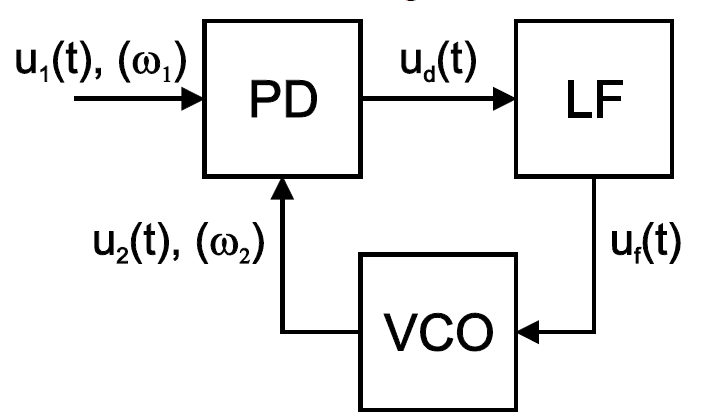
\includegraphics[width=0.9\textwidth]{images/Prinzip_PLL}\\
	\end{minipage}
	\begin{minipage}{0.55\textwidth}
	   Ein PLL ist ein Regelsystem, für die Phase $\varphi_1(t)$ und $\varphi_2(t)$. Das Ziel ist es, die Phase $\varphi_2(t)$ des  VCO's $\varphi_1(t)$ bis auf einen allfälligen (konstanten) Phasenfehler $\Delta \varphi_0$ nachzuregeln.\\
       Weil: $\varphi _1(t\to \infty ) - \varphi_2(t \to \infty)= \Delta \varphi = const$ und somit $\Delta \omega = \frac{d}{dt}\Delta \varphi_0 = 0$ ist, komm man zum Schluss, dass für die Frequenzen $\omega_1 = \omega_2$ gelten muss.
	\end{minipage}

    \begin{minipage}{0.50\textwidth} 
       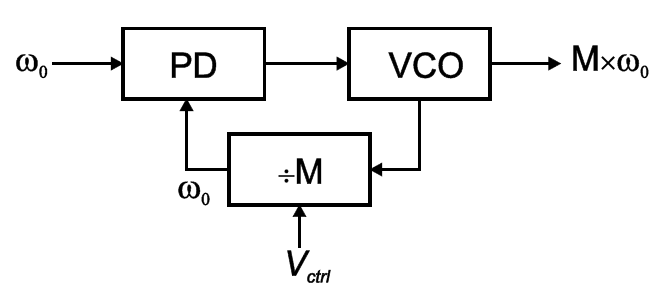
\includegraphics[width=0.9\textwidth]{images/Hohe_Frequ}\\
    \end{minipage}
    \begin{minipage}{0.4\textwidth}
      Vergleicht man das Referenzsignal mit einer durch einen Faktor M geteilten Teil des Oszillatorsignals, ist die Frequenz des Ausgangssignals um den Faktor M grösser als die des Eingangssignals. Wenn $M$ steuerbar ist, lassen sich exakte Vielfache der Frequenz ω0 erzeugen. Lässt sich ein rationales Teilerverhältnis N/M einstel-len, spricht man von einer "Fractional-N PLL". Mit speziellen Techniken kann man mit einem Fractional-N PLL kontinuierlich einstellbare Frequenzbereiche erzielen.
    \end{minipage}
\end{figure}

\subsection{VCO \normalfont{\small{(Skript S.7-5 (PLL))}}} 
\label{Kap.VCO}
\vspace{-0.7cm}
\begin{figure}[h!]
	\begin{minipage}{0.3\textwidth} 
       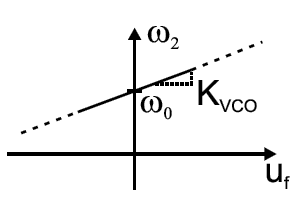
\includegraphics[width=0.7\textwidth]{images/K_VCO}
	\end{minipage}
	\begin{minipage}{0.6\textwidth}
	Aufgabe: Generierung einer Frequenz in Funktion einer Spannung
	   \begin{equation*}
         \begin{split}
            &\omega_2 = \omega_0+K_{VCO}\cdot u_f(t) \quad \quad (K_{VCO}=\text{VCO-Verstärkung})  \\
            &\varphi_2(t) =\int \limits_{t_0}^{t} \omega_2 \ d\tau =\int \limits_{t_0}^{t} \omega _0 + K_{VCO}\cdot u_f (\tau)\ d \tau =\omega_0 t + K_{VCO} \int \limits_{}^{} u_f(\tau) d\tau +\varphi_2_0 \\
         \end{split}
        \end{equation*}
	\end{minipage}
\end{figure}
\vspace{-0.7cm}

\subsection{Phasendetektor (PD) \normalfont{\small{(Skript S.7-6 (PLL))}}}
\label{Kap.VCO}
\vspace{-0.7cm}
\begin{figure}[h!]
	\begin{minipage}{0.2\textwidth} 
       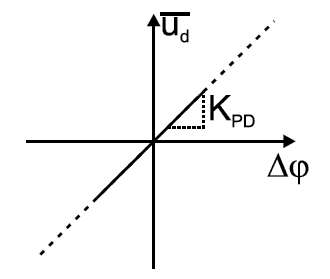
\includegraphics[width=1\textwidth]{images/Phasen_Detekt}
    \vspace{0.2cm}
	\end{minipage}
	\begin{minipage}{0.7\textwidth}
	   Aufgabe: Differenzbildner für die Phasensignale. Die mittlere Ausgangsspannung ist: 
	   \begin{equation*}
         \begin{split}
            \overline{u_d}=K_{PD}\cdot \Delta \varphi
         \end{split}
        \end{equation*}
        In der Praxis werden verschiedene Elemente eingesetzt:  \\  ($V_0$: max. Wert von $\overline{u_d}$)
	\end{minipage}
\end{figure}

\vspace{-1cm}
\begin{figure}[h!]
	\begin{minipage}{0.1\textwidth}
        \begin{tabular}{|c|c|c|c|}
          \hline
          Analoger Multipplizierer               & EXOR-Gatter                      & Flankengetriggertes JK-FF                            & Phasen-Frequenzdetektor (PFD)\\
          \hline \hline
          $K_{PD}=\frac{U_1 U_2}{2}\cdot \Delta$ & $K_{PD}=\frac{V_{0}}{\pi}$       & $K_{PD}=\frac{V_{0}}{\pi}=\frac{V_{DD}}{2\pi}$       & $K_{PD}=\frac{V_{0}}{2\pi}=\frac{V_{DD}}{4\pi}$ \\
          \hline
          für $\varphi \to 0 \ (<< 1 rad)$        & für $\Delta\varphi \in [0,\pi]$  & für $\Delta\varphi \in [-\pi,\pi]$                   & für $\Delta\varphi \in [-2\pi,2\pi]$ \\    
          (nichtlinear)                          & Abhängig von                     & nicht abhängig von                                   & 3 Zustände!\\
                                                 & Tastverhältnis!                  & Tastverhältnis!                                      &\\
          \hline
        \end{tabular}
	\end{minipage}
\end{figure}

\FloatBarrier
\subsection{Schleifenfilter} \normalfont{\small{(Skript S.7-10 (PLL))}}}
Aufgabe: Mitteln des PD-Signals (TP-Charakteristik). Dafür gibt es folgenden Methoden:
\begin{figure}[h!]
\begin{minipage}{0.1\textwidth}
        \begin{tabular}{|c|c|c|c|}
          \hline
          Loopfilter mit Charge-Pump *                            & EXOR-Gatter                       & passives Lag-Filter                                   & aktives Lag-Filter\\
          \hline \hline
          $H_{s}=\frac{I{pump}}{2 \cdot \pi \cdot C_p \cdot s}$   & $H_{s}=\frac{1}{1+s\tau}$         & $H_{s}=\frac{1+s\tau _2}{1+s(\tau _1 +\tau _2)}$      & $H_{s}=\frac{1+s\tau _2}{1\tau _1 }$  \\
          \hline
          +1: C aufladen                                          & einfach, oft ungenügend           &                                                       &\\    
          0: Wert behalten                                        & zusätzlich einen Pol              &                                                       & \\
          -1: C entladen                                          & $\to$ evt. Dämpfung zu klein      &                                                       &  \\
          \hline
        \end{tabular}
	\end{minipage}
\end{figure}
\FloatBarrier
* (für PFD) 

\FloatBarrier
\subsection{Linearisierung \normalfont{\small{(Skript S.7-12 (PLL))}}}
\begin{figure}[h!]
	\begin{minipage}{0.5\textwidth} 
       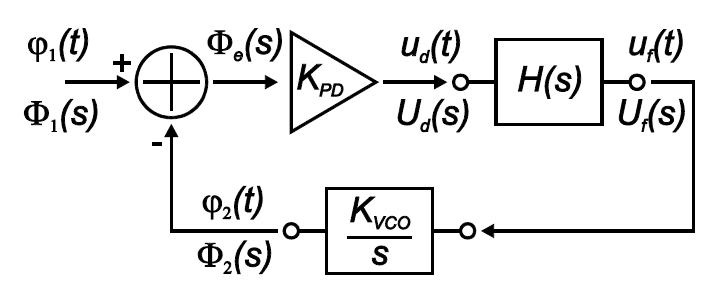
\includegraphics[width=1\textwidth]{images/linear_PLL}
	\end{minipage}
	\begin{minipage}{0.4\textwidth} 
       \begin{compactitem}
          \item Linearisierung gilt für eingerasteteten PLL ($\omega_1 = \omega_2$) und leichte Abweichung der Ruhelage
          \item lineare Systeme können mit Laplace-Transformation analysiert werden.
       \end{compactitem}
	\end{minipage}
\end{figure}

\FloatBarrier
\subsection{Eigenschaften der PLL im eingerasteten Zustand \normalfont{\small{(Skript S.7-12 (PLL))}}}
\begin{figure}[h!]
	\begin{minipage}{0.5\textwidth} 
       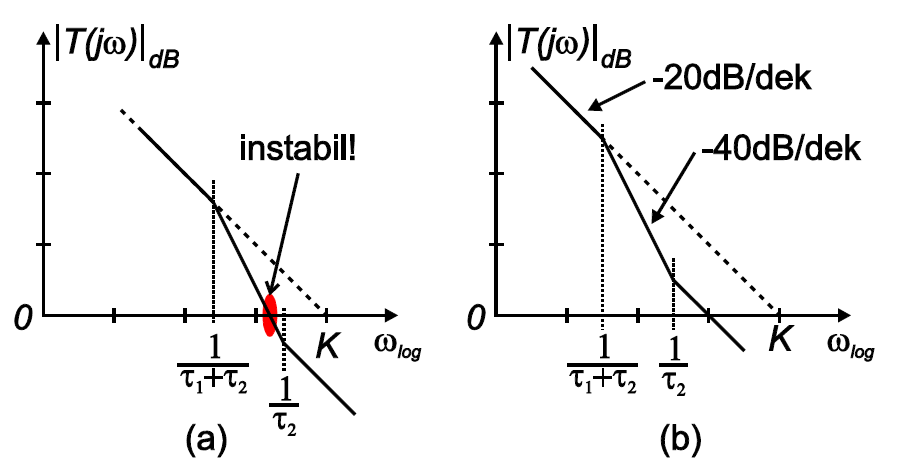
\includegraphics[width=1\textwidth]{images/PLL_Stabilitaet}
	\end{minipage}
	\begin{minipage}{0.4\textwidth} 
       \begin{compactitem}
          \item Stabilität ist wie bei anderen Regelkreisen wichtig. Sonst rastet PLL nicht ein.
          \item Nullstelle bei $s=\frac{1}{\tau_2}$ muss zu niedrigen Frequenzen verschoben werden, dass System stabil ist.
       \end{compactitem}
	\end{minipage}
\end{figure}

%\begin{figure}[h!]
       \begin{compactitem}
          \item \textbf{Haltebereich (hold range)} $\Delta \omega_H = V_{PD,max}\cdot H(0)\cdot K_{VCO}$: Ist der PLL eingerastet, so rastet er innerhalb des Haltebereichs nicht aus, solange es sich um statische (sehr langsame) Frequenzveränderungen handelt. 
          \item \textbf{Einrastbereich (pull-in range)} $\Delta \omega_{P}$: In diesem Bereich von Frequenzdifferenzen schafft es der PLL, wieder einzurasten. Der Einrastvorgang ist sehr langsam.
          \item \textbf{Ausrastbereich (pull-out range)} $\Delta \omega_{PO}$: Ist eine Frequenzschritt am Eingang der PLL grösser als ΔωPO, dann rastet der PLL aus.
          \item \textbf{Einrastbereich (lock-in range)} $\Delta \omega_{L} \approx 2 \zeta \omega_n$: Bei Frequenzveränderungen, die kleiner sind als ΔωL bleibt der PLL eingerastet. Das sollte der normale Arbeitsbereich eines PLLs sein. Es ist auch die maximale Frequenz, bei der das sofortige Einrasten (lock-in) möglich ist. ($\zeta:$ Dämpfung, $\omega_n$ = natürliche Frequenz.
          \item \textbf{Einrastzeit(lock-in time)} $T_{L} \approx \frac{2\pi}{\omega _n}$: Es ist die Zeit, für das Erreichen des eingerasteten Zustands 
        \end{compactitem}}
%\end{figure}

\FloatBarrier
\subsection{ADPLL (All Digital PLL)\normalfont{\small{(Skript S.7-1 (ADPLL))}}}
\begin{figure}[h!]
	\begin{minipage}{0.45\textwidth} 
       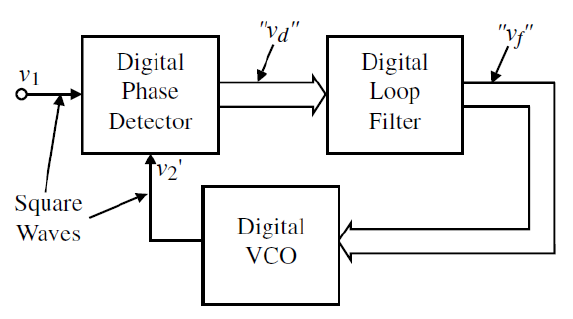
\includegraphics[width=1\textwidth]{images/ADPLL}
         \subcaption*{ADPLL}
	\end{minipage}
	\begin{minipage}{0.45\textwidth} 
       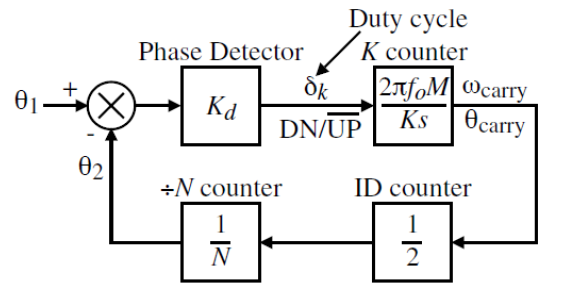
\includegraphics[width=1.1\textwidth]{images/linear_ADPLL}
         \subcaption*{Linearisierung ADPLL}
	\end{minipage}
\end{figure}

\begin{multicols}{2}
    \subsubsection{Phasendetektor}
    \begin{compactitem}
        \item \textbf{XOR}  
         \item \textbf{JK-FlipFlop} 
         \item \textbf{FF-Counter} $N$ von $0$ bis $\frac{T_{per}}{T_{clk}}$
         \item \textbf{Nyquist Rate Phase Detector}: Analoger Multiplizierer wird mit ADC und digitaler Multiplikation realisiert.
         \item \textbf{Zero-Crossing Phase Detector)}: Abtastung des Eingagssignals beim Nulldurchgang vom Feedback-Loop
         \item \textbf{Hilbert Transform Phase Detector)}
         \item \textbf{Digital-Averaging Phase Detector)}
    \end{compactitem}
    
    \subsubsection{Loop-Filter}
    \begin{compactitem}
         \item \textbf{\boldmath$N$ before \boldmath$M$ Loop Filter}  
         \item \textbf{UP/DOWN Counter Loop Filter} 
         \item \textbf{K Counter Loop Filter} 
         \item \textbf{Loop Filter mit \boldmath$N$-bit Parallel Input Signal}
    \end{compactitem}
    
    \subsubsection{Digital-kontrollierbarer Oszillator DCO}
    Realisierung (Programmierbare Frequenzteiler, spezielle Teiler):
    \begin{compactitem}
         \item \textbf{Programmierbarer Frequenzteiler}  
         \item \textbf{ID Counter} 
    \end{compactitem}
    Anwendungen: Skript S.7-11 (ADPLL)
\end{multicols}
